\documentclass[11pt,a4paper,UTF8,fontset=fandol]{ctexart}

\usepackage[margin=2.2cm]{geometry}
\usepackage{amsmath,amssymb,bm}
\usepackage{booktabs}
\usepackage{graphicx}
\usepackage{xcolor}
\usepackage[hidelinks]{hyperref}

\definecolor{DeepBlue}{HTML}{08306B}
\definecolor{BornBlue}{HTML}{2171B5}
\definecolor{AlertOrange}{HTML}{C65D07}

\ctexset{
    section={
        format=\Large\bfseries\color{DeepBlue},
        beforeskip=1.2ex plus 0.2ex,
        afterskip=0.6ex plus 0.1ex
    },
    subsection={
        format=\large\bfseries\color{BornBlue},
        beforeskip=0.9ex plus 0.2ex,
        afterskip=0.4ex plus 0.1ex
    }
}

\setlength{\parindent}{2em}
\setlength{\parskip}{0.25em}
\setlength{\abovedisplayskip}{0.55em}
\setlength{\belowdisplayskip}{0.55em}

\newcommand{\Tr}{\operatorname{Tr}}
\newcommand{\ee}{\mathrm e}

\title{有限温度 Born-sampling stoMPS 算法简介}
\author{}
\date{}

\begin{document}

\maketitle
\vspace{-2.5em}

\begin{abstract}
stoMPS 用一组随机对称矩阵乘积态近似热力学迹，但从无限温系综独立抽样时，
低温虚时演化会产生高度不均匀的样本权重。当前横场 Ising 实现先用
SETTN+tanTRG 构造有限温度 purification，再顺序测量其辅助物理腿，直接按照
Born 概率产生与目标热态匹配的 snapshot。这样可在切换逆温
$\beta_0$ 处消除额外的重要性权重，并只需继续演化
$\Delta\beta=\beta-\beta_0$。
\end{abstract}

\section{从随机迹估计到有限温度抽样}

传统 stoMPS 构造随机态 $|\xi\rangle$，使其系综平均满足
\begin{equation}
    \mathbb E_{\xi}\!\left[|\xi\rangle\langle\xi|\right]=cI .
\end{equation}
令 $|\xi_\beta\rangle=\ee^{-\beta H/2}|\xi\rangle$，有限温度观测量可写为
\begin{equation}
    \langle O\rangle_\beta=
    \frac{\mathbb E_{\xi}
    [\langle\xi_\beta|O|\xi_\beta\rangle]}
    {\mathbb E_{\xi}
    [\langle\xi_\beta|\xi_\beta\rangle]} .
    \label{eq:stochastic_trace}
\end{equation}
这个估计器本身是正确的，但 $|\xi\rangle$ 仍从 $\beta=0$ 的 proposal
中产生。随着温度降低，权重
$w_\xi=\langle\xi_\beta|\xi_\beta\rangle$ 会变得很宽，导致
$N_{\mathrm{eff}}\ll N_s$：大量样本几乎不贡献统计量。

\section{Purification Born snapshot}

在切换点 $\beta_0$，tanTRG 保存的是归一化热算符
\begin{equation}
    \bar R_{\beta_0}
    =\frac{\ee^{-\beta_0H/2}}{\sqrt{Z(\beta_0)}} ,
    \qquad
    \Tr\!\left(\bar R_{\beta_0}\bar R_{\beta_0}^{\dagger}\right)=1 .
\end{equation}
把 $\bar R_{\beta_0}$ 看成系统与辅助空间之间的 purification，并在一个完备
product basis $\{|a\rangle\}$ 中测量辅助腿。完整配置的 Born 概率及归一化
snapshot 为
\begin{equation}
    p(a)=\|\bar R_{\beta_0}|a\rangle\|^2,
    \qquad
    |\psi_a(\beta_0)\rangle
    =\frac{\bar R_{\beta_0}|a\rangle}{\sqrt{p(a)}} .
    \label{eq:born_snapshot}
\end{equation}
Born 抽样的核心恒等式是
\begin{align}
    \mathbb E_{a\sim p}
    [|\psi_a(\beta_0)\rangle\langle\psi_a(\beta_0)|]
    &=\sum_a \bar R_{\beta_0}|a\rangle
      \langle a|\bar R_{\beta_0}^{\dagger} \\
    &=\frac{\ee^{-\beta_0H}}{Z(\beta_0)}
    =\rho(\beta_0).
    \label{eq:density_reconstruction}
\end{align}
因此 $p(a)$ 已经由样本出现频率计入，不能再乘一次 $p(a)$ 或 $1/p(a)$。
每个归一化 snapshot 在 $\beta_0$ 处均以零初始相对 log weight 开始。

\subsection{顺序条件抽样}

程序不显式形成指数维的 $p(a)$，而是把 thermal MPO 正交中心移到第一个
site，并逐点执行：
\begin{enumerate}
    \item 将当前中心张量的 \texttt{physical\_in} 腿投影到每个允许的局域
    $Z_2$ sector；候选张量范数平方给出条件概率 $p(q_i|q_1,\ldots,q_{i-1})$；
    \item 按条件概率选择 $q_i$，归一化选中的候选张量；
    \item 把正交中心移动到下一个 site，使已抽取电荷通过虚拟 block 进入下一步
    条件环境。
\end{enumerate}
所有 site 完成后得到归一化 rank-4 MPS。被测量的局域电荷保存在一维
marker 腿中；thermal MPO 的左右虚拟腿没有被 collapse，因此 snapshot
通常仍是具有非平凡 bond dimension 的纠缠态，而不是 product state。

从 $\beta_0$ 到目标 $\beta$ 只需继续
\begin{equation}
    |\psi_a(\beta)\rangle
    =\ee^{-(\beta-\beta_0)H/2}|\psi_a(\beta_0)\rangle .
\end{equation}
后续归一化前的范数变化以 log weight 累积，热平均仍按式
\eqref{eq:stochastic_trace} 的加权比值计算。当前生产结果使用 exact/no-truncation
的 snapshot contraction；若启用有限 snapshot 压缩维度，还需要额外检查由压缩
引入的系统误差。

\section{\texorpdfstring{$Z_2$}{Z2} 对称性的含义}

当前模型采用 Pauli 矩阵约定
\begin{equation}
    H=-J\sum_{\langle i,j\rangle}\sigma_i^z\sigma_j^z
      -h\sum_i\sigma_i^x,
    \qquad
    P=\prod_i\sigma_i^x,
    \qquad [H,P]=0 .
\end{equation}
在 $X$ basis 中，$|+x\rangle$ 与 $|-x\rangle$ 分别对应局域
$Z_2$ 电荷 $q=0,1$。顺序 Born 测量每次选择一个一维 irrep，完整配置的
全局宇称为 $Q=\bigoplus_i q_i$。由于
$[\bar R_{\beta_0},P]=0$，得到的 snapshot 和随后的虚时演化都保持在对应的
全局宇称 sector 内。算法没有预先固定 even 或 odd；两类 sector 按各自的热权重
$Z_Q(\beta_0)/Z(\beta_0)$ 自然出现。

\clearpage
\section{数值结果：开放边界 \texorpdfstring{$10\times10$}{10 x 10} TFIM}

图~\ref{fig:comparison} 比较了 $J=1$、$h=3$、开放边界 $10\times10$
横场 Ising 模型的 SSE、直接 stoMPS、三个有限温度切换点的
tanTRG+stoMPS，以及纯 tanTRG。抽样曲线使用 $N_s=100$，张量网络参数为
$D=256$、$D_{\mathrm{SETTN}}=128$。上、中、下三个面板依次给出每格点能量、
相对 SSE 的绝对能量误差和每格点比热。

\begin{figure}[htbp]
    \centering
    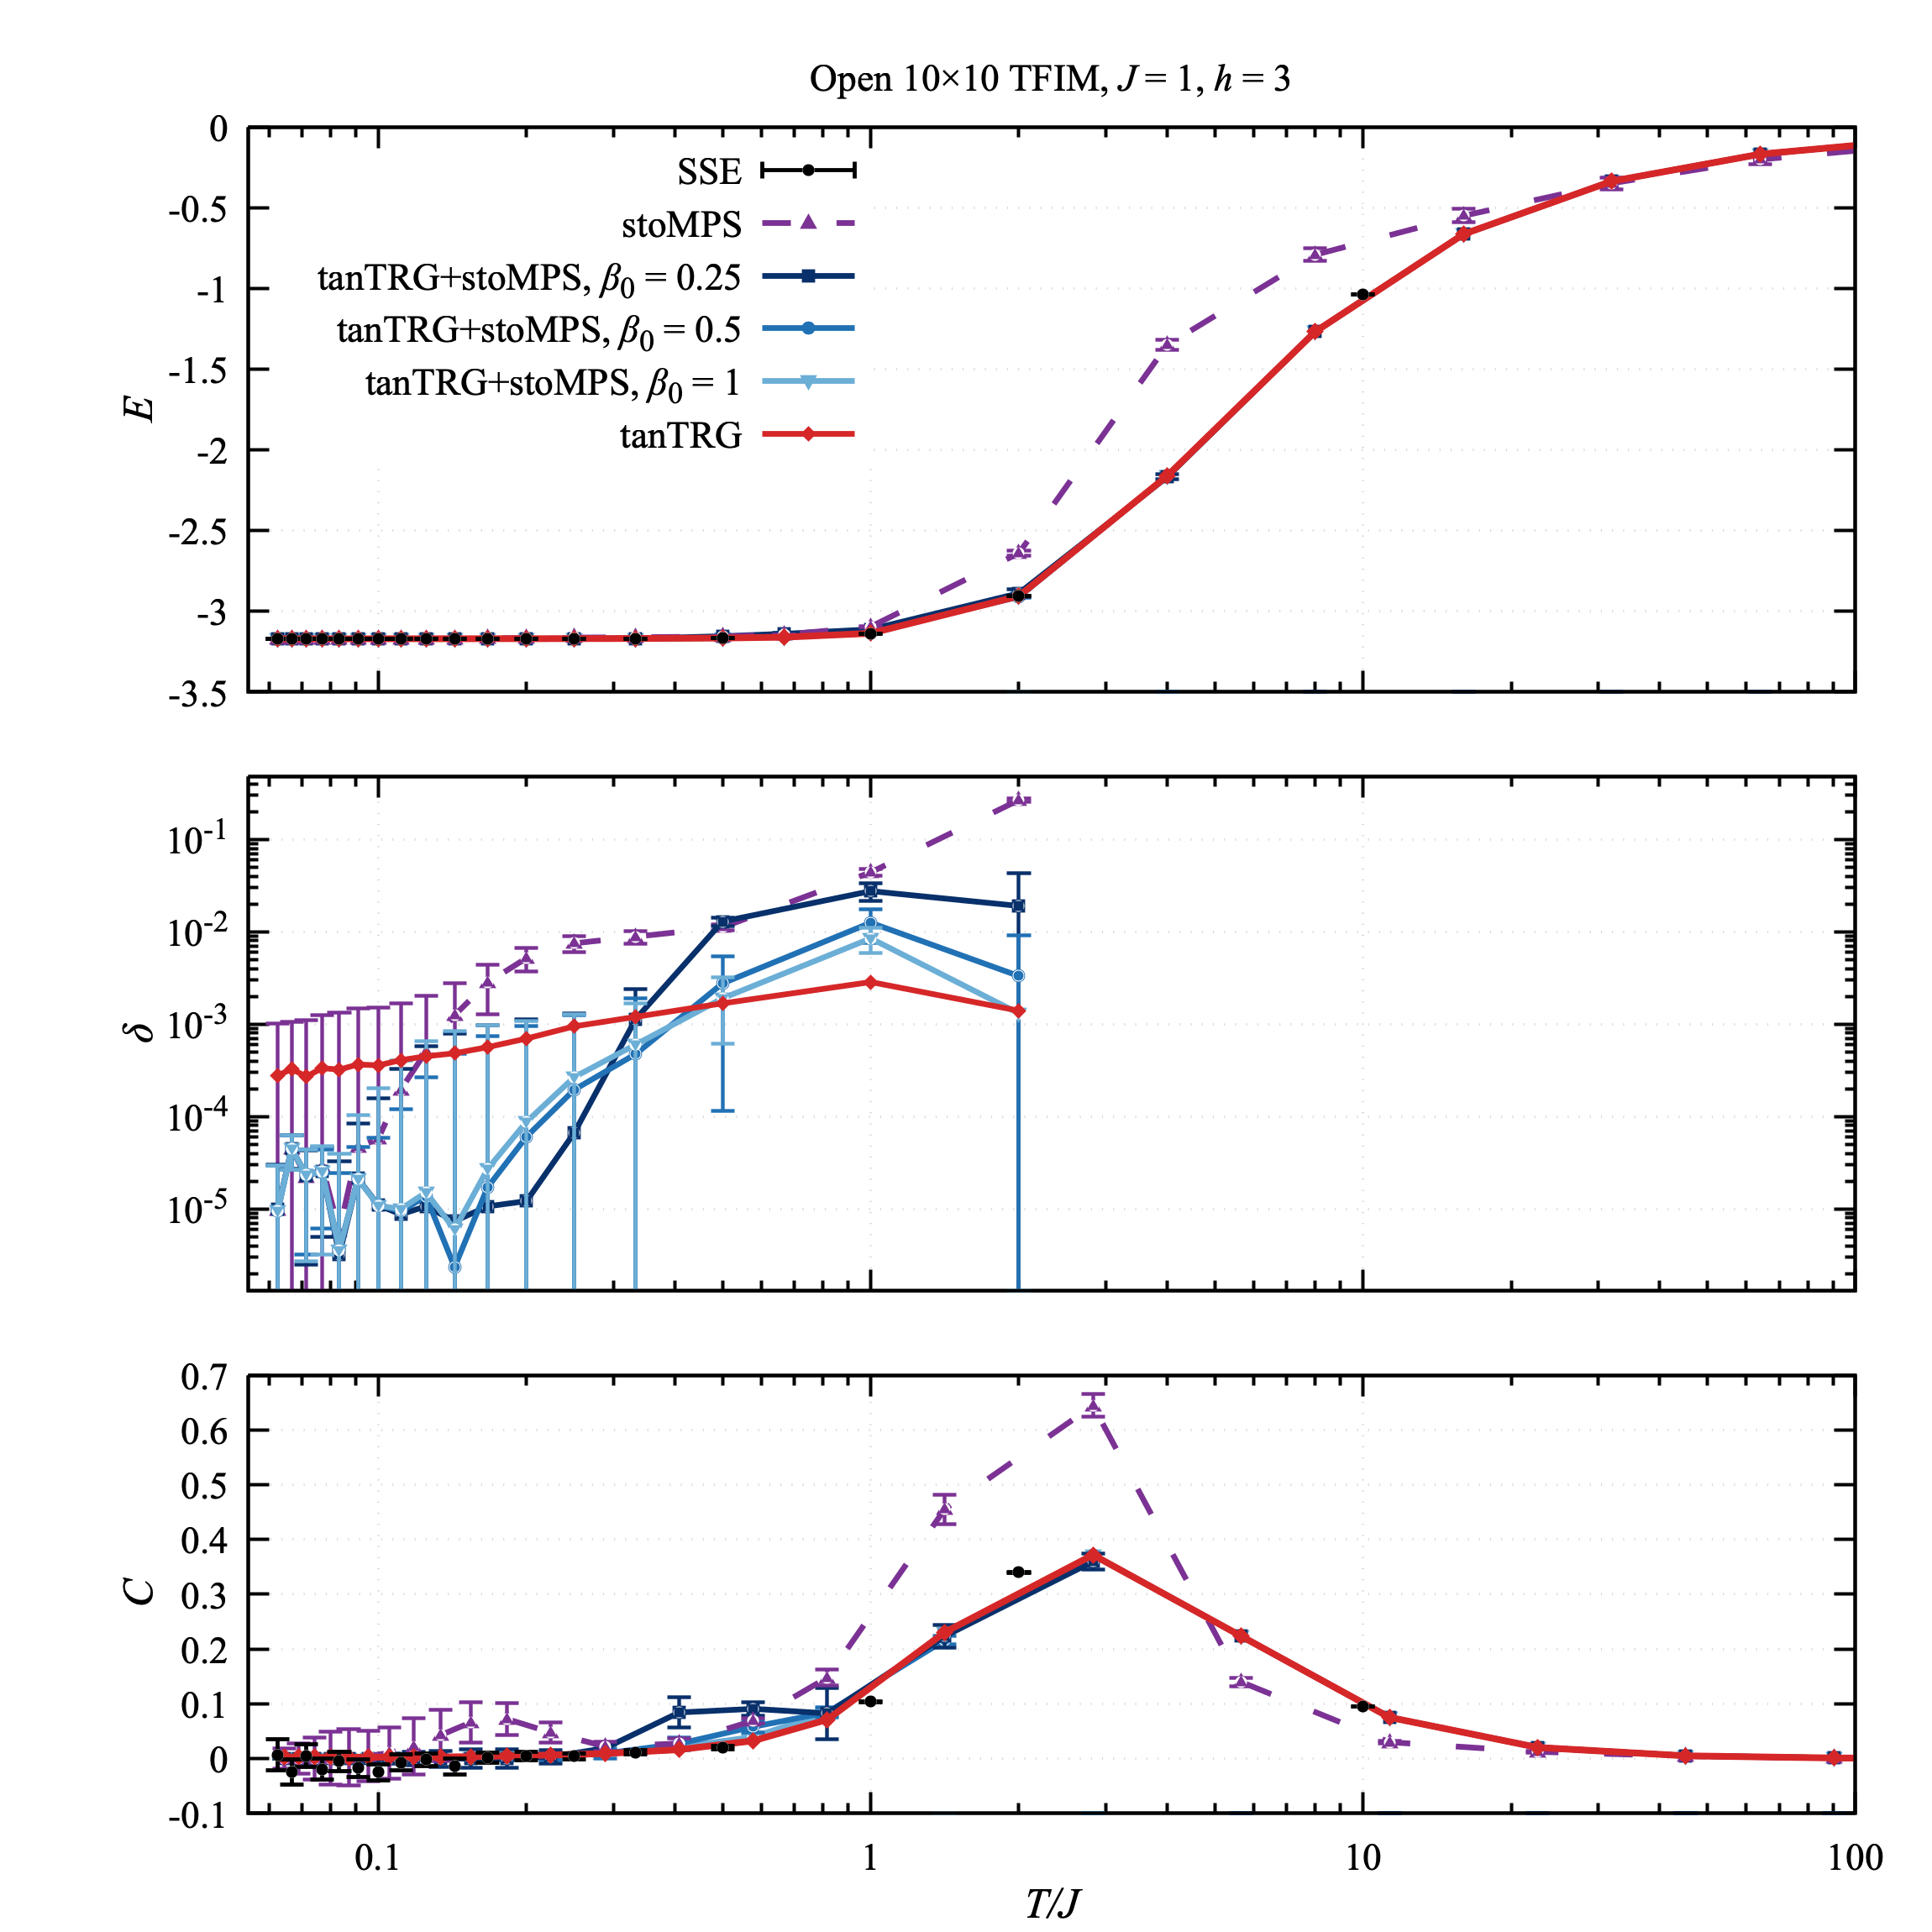
\includegraphics[width=0.88\textwidth]
        {tfim_open_10x10_h3_born_sse_comparison.png}
    \caption{开放边界 $10\times10$ TFIM 的有限温结果。直接从极高温开始的
    stoMPS 在中低温出现明显偏差；在有限 $\beta_0$ 从 thermal purification
    做 Born snapshot 后，混合方法的能量与 SSE/tanTRG 基准符合得更好。
    图中误差棒表示统计误差，不包含有限 bond dimension、tanTRG/TDVP
    截断或温度离散化等系统误差。}
    \label{fig:comparison}
\end{figure}

\paragraph{复现文件。}
\small
本文档、长表数据、绘图脚本和图像均位于同一目录。运行
\texttt{julia}\ \path{plot_tfim_open_10x10_h3_born_sse_comparison.jl}
即可从同目录 CSV 重新生成图~\ref{fig:comparison}，不需要读取原始 JLD2
样本或外部 SSE 文件。

\end{document}
